\section{Complementary Analysis Targeting Low Signal Masses}


\section{Combined Results}

\begin{figure}[htbp]
	\centering
	\subfigure[]{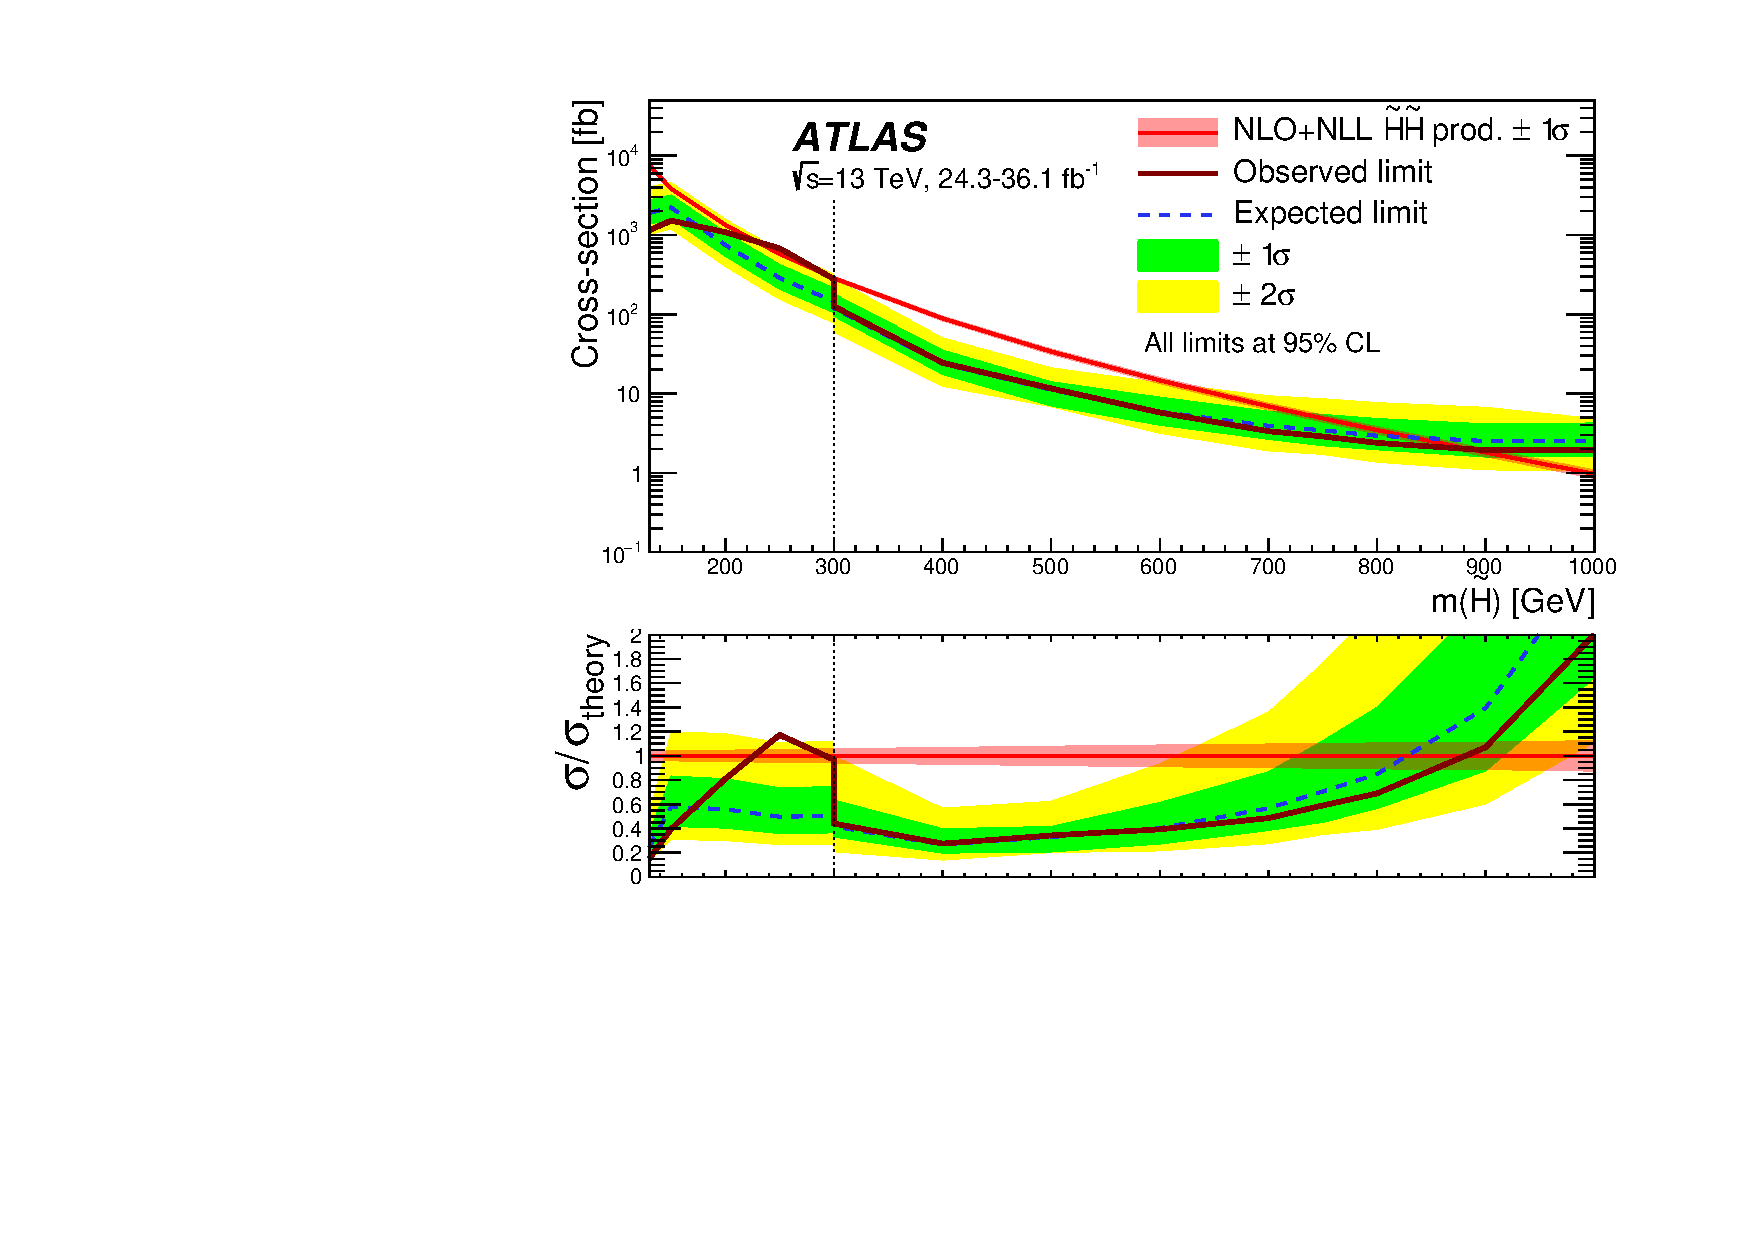
\includegraphics[width=0.75\textwidth]{figures/ewk_prod/interpretation/GGMupperLimit_unblinded_jump}\label{fig:exclusion_combined}}\\
	\subfigure[]{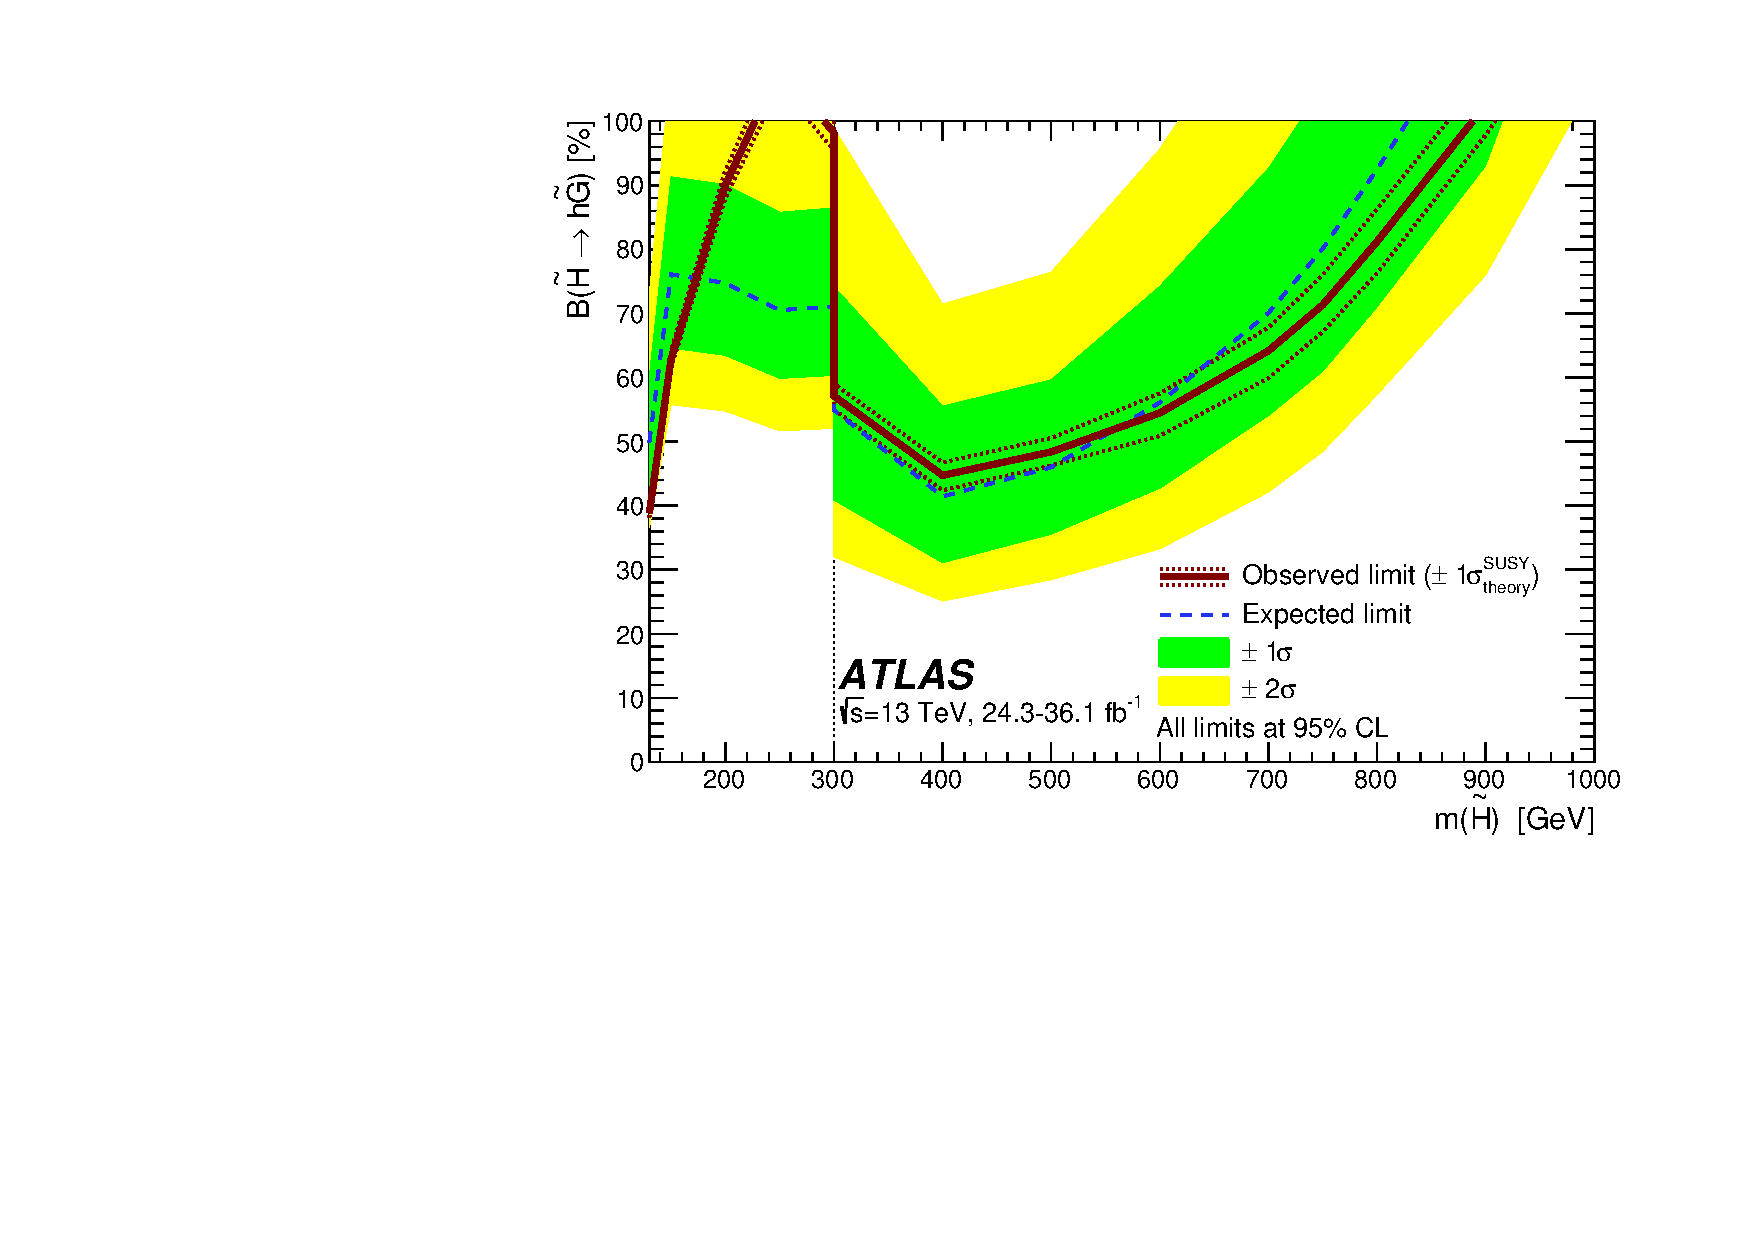
\includegraphics[width=0.75\textwidth]{figures/ewk_prod/interpretation/my_br_plot_unblind_yellow_band}\label{fig:exclusion_br}}
	\caption{Exclusion limits on \hino\ pair production. In both interpretations, the results of the low-mass analysis are used below $\mhino = 300$ GeV, while those of the high-mass analysis are used above. The figure shows (a) the observed (solid) vs expected (dashed) 95\% upper limits on the \hino\ pair production cross-section as a function of \mhino.  The 1$\sigma$ and 2$\sigma$ uncertainty bands on the expected limit are shown as green and yellow, respectively. The theory cross-section and its uncertainty are shown in the solid and shaded red curve. The bottom panel shows the ratio of the observed and expected limits with the theory cross-section. The figure also shows (b) the observed (solid) vs expected (dashed) 95\% limits in the \mhino\ vs $B(\hino\rightarrow h \tilde{G})$ plane, where $B(\hino\rightarrow h \tilde{G})$ denotes the branching ratio for the decay $\hino \rightarrow h \gravino$. The 1$\sigma$ uncertainty band is overlaid in green and the 2$\sigma$ in yellow. The regions above the lines are excluded by the analyses.} 
	\label{fig:exclusion}
\end{figure}
